\section{Definition of the species types and their state features}

In order to build multi-component multistate entities, one needs to define the building blocks that will be combined. A given type of component, a \class{SpeciesType},  can carry several \class{StateFeature}s, which are multi-valued characteristics of the component. One can also specify if instances of a \class{SpeciesType} can act as binding sites. Apart from a unique identifier, a name, and several annotations, it is furthermore possible to define state features of a component, and the values taken by those state features.  The following UML diagram shows how the structure of the \class{SpeciesType} looks like. 

\begin{figure}[H]
\begin{center}
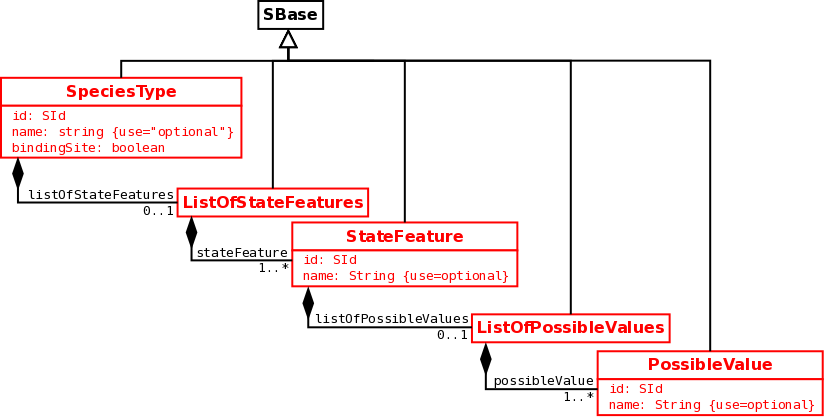
\includegraphics[scale=0.3]{figs/pngs/SpeciesTypeGeneral.png} 
\caption{\class{SpeciesType} and all the associated classes.}
\label{fig:SpeciesTypeGeneral}
\end{center}
\end{figure}

\subsection{SpeciesType} 

The element \class{SpeciesType}, which is part of \sbmlLtwoVfour specification, is not part of \sbmlLthreeVone any more. Instead, it will be defined in the \emph{multi} package. The \class{SpeciesType} element carries not only the basic attributes which it had in \sbmlLtwoVfour (\attribute{metaid}, \attribute{id}, \attribute{name}), but is also extended for the needs of describing multi-component entities with the attribute \attribute{bindingSite} and for the needs of multistate entities by linking it to a list of  \class{StateFeature}s.

\begin{figure}[H]
\begin{center}
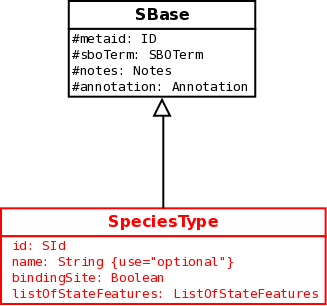
\includegraphics[scale=0.3]{figs/pngs/SpeciesTypeClass.png} 
\caption{Definition of \class{SpeciesType} and its relation with \class{SBase}.}
\label{fig:SpeciesTypeClass}
\end{center}
\end{figure}

A species type can be used to describe a component of a supra-macromolecular assembly, but also a domain of a macromolecule. Such a domain can be a portion of the macromolecule, a non-connex set of atoms forming a functional domain, or just a conceptual construct suiting the needs of the modeler. The type of component can be specified by referring terms from the subbranch \emph{functional entity} of the Systems Biology Ontology (\url{http://biomodels.net/sbo/}, \citep{Lenov:2007}) through the optional \attribute{sboTerm} attribute. The following table provides typical examples of component or domains (the list is absolutely not complete).\\

\begin{center}
\begin{tabular}{ll}
\hline
SBO identifier & definition \\
\hline
SBO:0000242 & channel \\
SBO:0000244 & receptor \\
SBO:0000284 & transporter \\
SBO:0000280 & ligand \\ 
SBO:0000493 & functional domain \\
SBO:0000494 & binding site \\
SBO:0000495 & catalytic site \\
SBO:0000496 & transmembrane domain \\
\hline
\end{tabular}\\[\baselineskip]
\end{center}

The example below encodes a species type representing a ligand-gated ion channel, that is a transmembrane macromolecule that can form a ionic channel stabilised by the binding of ligands. Notice the notes and annotation that belong to the namespace of \sbmlLthreeVone \emph{core}.

\begin{example}
<multi:speciesType xmlns:core="http://www.sbml.org/sbml/level3/version1"
                   xmlns:multi="http://www.sbml.org/sbml/level3/version1/multi/version1" 
                   xmlns:xhtml="http://www.w3.org/1999/xhtml"
                   xmlns:rdf="http://www.w3.org/1999/02/22-rdf-syntax-ns#" 
                   xmlns:bqbiol="http://biomodels.net/biology-qualifiers/"
                   multi:id="speciesType1"
                   multi:name="LGIC"
                   multi:bindingSite="false" 
                   multi:sboTerm="SBO:0000242">
  <core:notes>
    <xhtml:body>
      <xhtml:p>LGIC is a Ligand-Gated Ion Channel</xhtml:p>
    </xhtml:body>
  </core:notes>
  <core:annotation>
    <rdf:RDF>
      <rdf:Description rdf:about="#_000003">
        <bqbiol:isVersionOf>
          <rdf:Bag>
            <rdf:li rdf:resource="urn:miriam:interpro:IPR002394"/>
          </rdf:Bag>
        </bqbiol:isVersionOf>
      </rdf:Description>
    </rdf:RDF>
  </core:annotation>
  <multi:listOfStateFeatures>
    <!-- some state features -->
  </multi:listOfStateFeatures>
</multi:speciesType>
\end{example}

The example below encodes a species type representing the binding site for a ligand, that could be used for instance in conjunction with the previous example. 

\begin{example}
<multi:speciesType xmlns:multi="http://www.sbml.org/sbml/level3/version1/multi/version1" 
                   multi:id="speciesType2"
                   multi:name="AgonistSite" 
                   multi:bindingSite="true" 
                   multi:sboTerm="SBO:0000494" />
\end{example}

\subsection{StateFeature} 

A species type can carry any number of state features, which are characteristic properties specific for this type of species. The element \class{StateFeature} of \sbmlLthreeVone \multiVone corresponds to the ``state variable'' of the SBGN Entity Relationship language. A \class{StateFeature} is identified by an \attribute{id} and an optional \attribute{name}. A \class{StateFeature} is linked to a list of \class{PossibleValue}s.

\begin{figure}[H]
\begin{center}
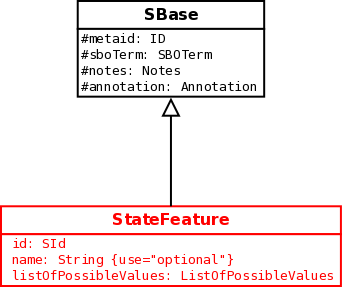
\includegraphics[scale=0.3]{figs/pngs/StateFeatureClass.png} 
\caption{Definition of \class{StateFeatureClass} and its relation with \class{SBase}.}
\label{fig:StateFeatureClass}
\end{center}
\end{figure}

As all elements derived from \class{SBase}, \class{StateFeature} can link to \class{Notes} and \class{Annotation}, and carry a \attribute{metaid}, and an \attribute{sboTerm}. The value \cdata{SBO:0000497} of \attribute{sboTerm} used in the example below corresponds to a ``ternary switch''.

%% Add notes and annotations below
\begin{example}
<multi:stateFeature 
              xmlns:multi="http://www.sbml.org/sbml/level3/version1/multi/version1" 
              multi:id="stateFeature1"
              multi:name="pore"
              multi:sboTerm="SBO:0000497">
  <multi:listOfPossibleValues>
    <!-- some possible values -->
  </multi:listOfPossibleValues>
</multi:stateFeature>
\end{example}

\subsection{PossibleValue}

Each state feature also requires the definition of all the possible values it can take. Those values will be used within a selector, to define the states an entity is allowed to take. A state feature is not obligatory a boolean property, but can carry any number of \class{PossibleValue}. A \class{PossibleValue} is identified by an \attribute{id} and an optional \attribute{name}.

\begin{figure}[H]
\begin{center}
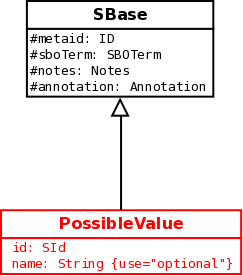
\includegraphics[scale=0.3]{figs/pngs/PossibleValueClass.png} 
\caption{Definition of \class{PossibleValue} and its relation with \class{SBase}.}
\label{fig:PossibleValueClass}
\end{center}
\end{figure}

As all elements derived from \class{SBase}, \class{PossibleValue} can link to \class{Notes} and \class{Annotation}, and carry a \attribute{metaid}, and an \attribute{sboTerm}. The \attribute{sboTerm} used in the example below corresponds to a ``ternary switch''. 

\begin{example}
<multi:possibleValue 
                     xmlns:multi="http://www.sbml.org/sbml/level3/version1/multi/version1" 
                     multi:id="possibleValue1" 
                     multi:name="open"
                     multi:sboTerm="0000416" />
\end{example}

\subsection{Complete definition of a species type}

The following example describes the SpeciesType presented on \fig{st_receptor}.

\begin{example}
<multi:speciesType xmlns:core="http://www.sbml.org/sbml/level3/version1"
                   xmlns:multi="http://www.sbml.org/sbml/level3/version1/multi/version1" 
                   xmlns:xhtml="http://www.w3.org/1999/xhtml"
                   xmlns:rdf="http://www.w3.org/1999/02/22-rdf-syntax-ns#" 
                   xmlns:bqbiol="http://biomodels.net/biology-qualifiers/"
                   multi:id="speciesType1"
                   multi:bindingSite="false" 
                   multi:name="LGIC" 
                   multi:sboTerm="SBO:0000242">
  <core:notes>
    <xhtml:body>
      <xhtml:p> 
        LGIC is a Ligand-Gated Ion Channel. It contains a pore that can be open or closed.
      </xhtml:p>
    </xhtml:body>
  </core:notes>
  <core:annotation>
    <rdf:RDF>
      <rdf:Description rdf:about="#_000003">
        <bqbiol:isVersionOf>
          <rdf:Bag>
            <rdf:li rdf:resource="urn:miriam:interpro:IPR002394"/>
          </rdf:Bag>
        </bqbiol:isVersionOf>
      </rdf:Description>
    </rdf:RDF>
  </core:annotation>
  <multi:listOfStateFeatures>
    <multi:stateFeature multi:id="stateFeature1"
                        multi:name="pore"
                        multi:sboTerm="SBO:0000497">
      <multi:listOfPossibleValues>
        <multi:possibleValue id="possibleValue1"
                             multi:name="open"
                             multi:sboTerm="SBO:0000416" />
        <multi:possibleValue id="possibleValue2"
                             multi:name="closed"
                             multi:sboTerm="SBO:0000417" />
        <multi:possibleValue id="possibleValue3"
                             multi:name="desensitised"
                             multi:sboTerm="SBO:0000417" />
      </multi:listOfPossibleValues>
    </multi:stateFeature>
  </multi:listOfStateFeatures>
</multi:speciesType>
\end{example}
